\chapter[Resultados]{Resultados}

\section{Análise teórica vs. Otimização do painel reforçado}
Esta seção está dividida em três subseções:
\begin{itemize}
\item Resultados da análise teórica do painel reforçado;
\item Resultados da otimização do painel reforçado fabricado em material metálico;
\item Comparação dos dois itens ateriores .
\end{itemize}

\subsection{Análise teórica do painel reforçado}
A análise teórica do painel reforçado seguiu a metodologia do \emph{Fator de Eficiência de Farrar} proposta por \cite{niu1997airframe}. O painel reforçado foi submetido a uma carga de compressão de intensidade 10000daN (22480lbs), obtendo-se portando uma carga de compressão linear (N) como segue:\\~\\

\centerline{N = 833,3 N/mm = 4758,5 lbs/in}\


Utilizou-se os valores otimizados na análise teórica:
F=0.81; $R_t$=2.25; $R_b$=0.65;
Da \autoref{fig_plotFarrar}, encontrou-se o valor de "f" correspondente a carga por largura (4758,5 lbs/in), utilizando F=0.81 para o Al 2024-T3 extrudado.\\~\\


\centerline{f = 41000 psi}\

Encontrou-se o módulo tangente $E_t$ correspondente ao valor de "f", da curva de módulo tangente do material, conforme \autoref{fig_tangentmodulus}.\\~\\

\centerline{$E_t$ = 5.0x$10^6$ psi}
\

Conforme \autoref{Farrar_Efficiency_t} e \autoref{Farrar_Efficiency_tw}, determinou-se os valores de $t$ e $t_w$.\\~\\

\centerline{$t = 0.501({\dfrac{NL}{E_t}})^{0.5} = 0.06 in = 1.524 mm$}\

\centerline{$t_w = 2.25t = 0.136in = 3.454 mm$}\


\subsection{Otimização do painel reforçado em material metálico}
Desenvolveu-se um modelo de otimização do reforçador em material metálico, no qual, o material possuia as mesma propriedade de módulo de elasticidade (E) do modelo teórico. Para este modelo, encontrou-se o seguinte resultado:\

\centerline{$t = 1.329 mm$}\

\centerline{$t_w = 3.447 mm$}\

\begin{figure}[ht]
 \caption{\label{fig_ModelMetallic}Resultado do reforçador em material metálico.}
 \centering
 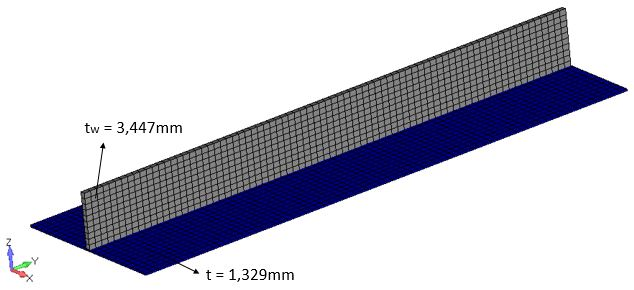
\includegraphics[scale=1.0]{figura/Model_Metallic1}
\end{figure}
\

\subsection{Comparação dos resultados}
A tabela seguinte compara os resultados das espessuras do revestimento e do reforçador obtidas na análise do modelo teórico e do modelo otimizado.
\begin{table}[h]
\centering
\begin{tabular}{ccc}
\toprule
Modelo & Espessura do revestimento (mm) & Espessura do reforçador (mm) \\\midrule
Teórico & 1.524 & 3.454\\
Otimizado & 1.329 & 3.447\\
\bottomrule
\end{tabular}
\caption{Resultados de espessuras.}
\label{tbl:result1_metalico}
\end{table}

Tendo-se como base a geometria do reforçador e a densidade mássica do material considerado, calculou-se as massas das estruturas. E os resultados são conforme mostrado na tabela seguinte.

\begin{table}[h]
\centering
\begin{tabular}{cc}
\toprule
Modelo & Massa (kg) \\ \midrule
Teórico & 0.353\\
Otimizado & 0.327\\
\bottomrule
\end{tabular}
\caption{Resultados de massa da estrutura.}
\label{tbl:result2_metalico}
\end{table}

Observa-se que foram encontradas espessuras, e consequentemente, massas das estruturas diferentes, entre os modelos teóricos e o modelo da otimização.
Em relação as espessuras, as diferenças entre os modelos foram de 12.79\% para o revestimento e 0.20\% para o reforçador, e em relação as massas de 7.37\%. Essas diferenças se devem ao fato de o modelo teórico ter considerado um reforçador ótimo com o fator de eficiência de Farrar de 0.81, e caso esse fator pudesse ser melhorado, o modelo teórico ficaria mais aproximado do modelo otimizado.

\section{Análise teórica vs. Otimização do painel reforçado}
Esta seção está dividida em três subseções:
\begin{itemize}
\item Resultados da otimização do painel reforçado fabricado em material metálico;
\item Resultados da otimização do painel reforçado fabricado em material composto;
\item Comparação dos dois itens ateriores .
\end{itemize}

\subsection{Otimização do painel reforçado em material metálico}

\subsection{Otimização do painel reforçado em material composto}

\subsection{Comparação dos resultados}
